%% Преамбула TeX-файла

% 1. Стиль и язык
\documentclass{G7-32} % Стиль (по умолчанию размер шрифта 14pt)

% Стандартные настройки убраны в preamble.inc.tex.
\sloppy

% Настройки стиля ГОСТ 7-32
% Для начала определяем, хотим мы или нет, чтобы рисунки и таблицы нумеровались в пределах раздела, или нам нужна сквозная нумерация.
\EqInChapter % формулы будут нумероваться в пределах раздела
\TableInChapter % таблицы будут нумероваться в пределах раздела
\PicInChapter % рисунки будут нумероваться в пределах раздела

% Добавляем гипертекстовое оглавление в PDF
\usepackage[
bookmarks=true, colorlinks=true, unicode=true,
urlcolor=black,linkcolor=black, anchorcolor=black,
citecolor=black, menucolor=black, filecolor=black,
]{hyperref}

\AfterHyperrefFix

\usepackage{microtype}% полезный пакет для микротипографии, увы под xelatex мало чего умеет, но под pdflatex хорошо улучшает читаемость

% Тире могут быть невидимы в Adobe Reader
\ifInvisibleDashes
\MakeDashesBold
\fi

\usepackage{graphicx}   % Пакет для включения рисунков

% С такими оно полями оно работает по-умолчанию:
% \RequirePackage[left=20mm,right=10mm,top=20mm,bottom=20mm,headsep=0pt,includefoot]{geometry}
% Если вас тошнит от поля в 10мм --- увеличивайте до 20-ти, ну и про переплёт не забывайте:
\geometry{right=20mm}
\geometry{left=30mm}
\geometry{bottom=20mm}
\geometry{ignorefoot}% считать от нижней границы текста


% Пакет Tikz
\usepackage{tikz}
\usetikzlibrary{arrows,positioning,shadows}

% Произвольная нумерация списков.
\usepackage{enumerate}

% ячейки в несколько строчек
\usepackage{multirow}

% itemize внутри tabular
\usepackage{paralist,array}

%\setlength{\parskip}{1ex plus0.5ex minus0.5ex} % разрыв между абзацами
\setlength{\parskip}{1ex} % разрыв между абзацами
\usepackage{blindtext}

% Центрирование подписей к плавающим окружениям
\usepackage[justification=centering]{caption}

\usepackage{newfloat}
\DeclareFloatingEnvironment[
placement={!ht},
name=Equation
]{eqndescNoIndent}
\edef\fixEqndesc{\noexpand\setlength{\noexpand\parindent}{\the\parindent}\noexpand\setlength{\noexpand\parskip}{\the\parskip}}
\newenvironment{eqndesc}[1][!ht]{%
    \begin{eqndescNoIndent}[#1]%
\fixEqndesc%
}
{\end{eqndescNoIndent}}




% Настройки листингов через minted.
\usepackage{local-minted}

% Полезные макросы листингов.
% Любимые команды
\newcommand{\Code}[1]{\texttt{#1}}


% Стиль титульного листа кафедры ИТАС
\usepackage{title-petrenko}

% --- Заполняем данные для титульника ---
\LabNumber{4} % Номер лабораторной работы
\LabTopic{Реализация команд DDL, DML и соединений на веб-странице} % Тема работы
\LabStudent{РИС-25-2б}{Ильинов Ф. М.} % Группа и ФИО студента

\begin{document}

\begin{titlepage}
\end{titlepage}

\frontmatter % выключает сквозную нумерацию для вводной части

\tableofcontents

\mainmatter % включает арабскую нумерацию глав и разделов

\chapter{Цель работы}
\label{cha:aim}

Реализовать веб-приложение для взаимодействия с СУБД PostgreSQL, обеспечивающее выполнение полного жизненного цикла операций с реляционной базой данных:
\begin{enumerate}
    \item Команды DDL: создание, модификация, очистка и удаление таблиц;
    \item Команды DML: вставка, обновление и удаление;
    \item Команды SELECT и INNER JOIN ... ON);
\end{enumerate}

\chapter{Задачи работы}
\label{cha:tasks}

В соответствии с целью были поставлены следующие задачи:

\begin{enumerate}
    \item Разработать локальный веб-сервер на языке Golang (версия 1.27) с использованием стандартной библиотеки \texttt{net/http};
    \item Реализовать подключение к СУБД PostgreSQL с использованием пула соединений \texttt{pgx};
    \item Разработать механизм безопасной трансляции параметров пользовательских форм в команды SQL с экранированием;
    \item Реализовать стек вызовов для команд DDL;
    \item Реализовать стек вызовов для команд DML;
    \item Реализовать стек вызовов для выборок и соединений: построитель запросов SELECT и оператор соединения INNER JOIN по ключевым полям;
    \item Разработать веб-интерфейс на основе Server-Side Rendering (пакет \texttt{html/template}) с выводом результатов и текста выполненного SQL-запроса на страницу браузера.
\end{enumerate}

\chapter{Этапы выполнения}
\label{cha:stages}

Для выполнения поставленных задач были сформулированы следующие технологические требования к инструментарию:
\begin{itemize}
    \item Поддержка реляционной модели данных и стандарта SQL в СУБД PostgreSQL~\cite{doc:postgres,doc:sql};
    \item Поддержка сетевого протокола передачи гипертекста HTTP~\cite{wiki:http};
    \item Возможность отрисовки форм, кнопок и динамических таблиц в веб-интерфейсе.
\end{itemize}

Для реализации клиентского интерфейса был выбран язык разметки HTML~\cite{wiki:html} совместно с библиотекой стилей Pico CSS~\cite{wiki:pico.css}, обеспечивающей лаконичное визуальное оформление без необходимости написания сложного клиентского JavaScript-кода.

В качестве языка серверной части выбран Golang версии 1.27~\cite{wiki:go}. Для взаимодействия с СУБД PostgreSQL задействован драйвер и пул соединений \texttt{github.com/jackc/pgx}~\cite{git:pgx}.

Сервер функционирует по принципу Server-Side Rendering (SSR). Все страницы собираются на стороне сервера с помощью встроенного шаблонизатора \texttt{html/template} и возвращаются браузеру в виде готового HTML-документа.

\section{Архитектура веб-приложения и стек вызовов}
\label{sec:architecture}

Веб-приложение построено по многоуровневой схеме. Прохождение любого пользовательского действия организовано в виде строгого сквозного стека вызовов:
\begin{enumerate}
    \item клиентский уровень: веб-страница браузера (HTML-формы с параметрами операций DDL, DML или DQL);
    \item уровень веб-сервера и маршрутизации: маршрутизатор стандартной библиотеки Golang (версия 1.27), диспетчеризация по HTTP-методу и пути, распаковка параметров формы;
    \item уровень сборщика запросов (Query Builder): экранирование идентификаторов PostgreSQL двойными кавычками (\texttt{quoteIdent}) и строковых литералов одинарными кавычками (\texttt{quoteLiteral});
    \item уровень СУБД PostgreSQL: выполнение запроса через пул соединений \texttt{pgx}, опрос системного каталога \texttt{information\_schema};
    \item уровень представления (View Renderer): динамическое сканирование кортежей и отрисовка HTML-шаблона с отображением текста выполненного SQL-запроса и полученных данных.
\end{enumerate}

\subsection{Веб-сервер и маршрутизация запросов}

Инициализация сетевого мультиплексора и регистрация маршрутов выполняются в функции \texttt{main} (листинг~\ref{lst:main-router}).

\begin{listing}[H]
    \gofile[firstline=70, lastline=105, firstnumber=70]{../main.go}
    \caption{Маршрутизация HTTP-запросов DDL, DML и DQL в \texttt{main.go}}
    \label{lst:main-router}
\end{listing}

В строке 73 шаблон \texttt{"GET /\{\$\}"} задает строгое соответствие корневому пути и выполняет перенаправление на страницу таблиц \texttt{/tables}. Для остальных операций предусмотрено четкое разделение:
\begin{itemize}
    \item \texttt{GET}-запросы отображают страницы и формы (например, \texttt{/ddl/\{op\}}, \texttt{/dml/\{op\}}, \texttt{/select});
    \item \texttt{POST}-запросы принимают данные форм и запускают сборку и выполнение соответствующих SQL-команд (\texttt{/ddl/create}, \texttt{/dml/insert}, \texttt{/query/select} и др.).
\end{itemize}

\subsection{Архитектура обработчиков и обработка ошибок}

Для унификации обработки ошибок используется тип-адаптер \texttt{AppHandler} (листинг~\ref{lst:app-handler}), представляющий собой функцию, возвращающую ошибку.

\begin{listing}[H]
    \gofile[firstline=131, lastline=173, firstnumber=131]{../views.go}
    \caption{Структура \texttt{AppError} и адаптер обработчиков \texttt{AppHandler}}
    \label{lst:app-handler}
\end{listing}

Метод \texttt{ServeHTTP} перехватывает ошибки выполнения. Если возвращена ошибка \texttt{AppError}, фиксируется запись в логе и клиенту отправляется соответствующий HTTP-статус. При возникновении ошибки на уровне СУБД форма рендерится повторно со статусом \texttt{400 Bad Request}, сохраняя введенные пользователем значения и подсвечивая сообщение сервера PostgreSQL и проблемный SQL-запрос.

\subsection{Движок представления и шаблонизация}

Генерация веб-интерфейса реализована на стороне сервера с помощью встроенного пакета \texttt{html/template} и обертки \texttt{ViewRenderer} (листинг~\ref{lst:view-renderer}).

\begin{listing}[H]
    \gofile[firstline=14, lastline=39, firstnumber=14]{../views.go}
    \caption{Инициализация и рендеринг шаблонов в \texttt{views.go}}
    \label{lst:view-renderer}
\end{listing}

При запуске сервера компилируется базовый шаблон \texttt{layout.html}, после чего методом \texttt{Clone()} создаются изолированные копии для каждой рабочей страницы (\texttt{tables}, \texttt{ddl}, \texttt{dml}, \texttt{select}, \texttt{join}). Для динамических вычислений в разметке зарегистрированы специальные функции (листинг~\ref{lst:func-map}).

\begin{listing}[H]
    \gofile[firstline=44, lastline=60, firstnumber=44]{../main.go}
    \caption{Пользовательские функции шаблонизатора \texttt{funcMap}}
    \label{lst:func-map}
\end{listing}

Функции \texttt{seq} и \texttt{add} используются для циклической генерации динамических строк формы (например, добавление заданного количества колонок в DDL или кортежей в DML). Функция \texttt{getRowVal} обеспечивает безопасное извлечение сохраненных значений полей при повторной отрисовке после ошибок.

Базовый шаблон \texttt{layout.html} (листинг~\ref{lst:layout-html}) содержит навигацию, кнопку быстрого сброса БД и блок отображения сгенерированного SQL-запроса. Для предотвращения выхода широких таблиц за границы страницы контейнерам \texttt{figure} назначен стиль горизонтальной прокрутки \texttt{overflow-x: auto}.

\begin{listing}[H]
    \htmlfile[firstline=16, lastline=46, firstnumber=16]{../templates/layout.html}
    \caption{Разметка контейнера и блок аудита SQL в \texttt{layout.html}}
    \label{lst:layout-html}
\end{listing}

В строках 34--41 размещен блок уведомления об ошибках: если сервер СУБД возвращает ошибку, точный текст сформированного запроса выводится в теге \texttt{<pre><code>}.

\subsection{Пул соединений и взаимодействие с PostgreSQL}

Подключение к СУБД осуществляется в функции \texttt{main} через пул соединений библиотеки \texttt{pgx} (листинг~\ref{lst:db-pool}).

\begin{listing}[H]
    \gofile[firstline=25, lastline=37, firstnumber=25]{../main.go}
    \caption{Инициализация пула соединений \texttt{pgx}}
    \label{lst:db-pool}
\end{listing}

Пул соединений повторно использует открытые TCP-сессии к PostgreSQL, снижая накладные расходы на постоянную аутентификацию и установление соединения при каждом HTTP-запросе.

\subsection{Механизм безопасной сборки SQL-запросов}

Поскольку имена таблиц и столбцов передаются из веб-интерфейса динамически, прямое использование позиционных плейсхолдеров PostgreSQL (\texttt{\$1, \$2}) для них неприменимо. Для защиты от внедрения вредоносного SQL-кода (SQL Injection) в файле \texttt{db.go} реализованы специализированные функции экранирования (листинг~\ref{lst:quote-helpers}).

\begin{listing}[H]
    \gofile[firstline=39, lastline=45, firstnumber=39]{../db.go}
    \caption{Функции экранирования идентификаторов и литералов}
    \label{lst:quote-helpers}
\end{listing}

Функция \texttt{quoteIdent} экранирует идентификаторы PostgreSQL (имена таблиц, колонок) согласно стандарту: имя оборачивается в двойные кавычки, а внутренние кавычки удваиваются (\texttt{""}). Функция \texttt{quoteLiteral} обрамляет пользовательские строковые константы в одинарные кавычки с удвоением внутренних одинарных кавычек.

\section{Динамическое получение метаданных PostgreSQL и просмотр таблиц}
\label{sec:introspection}

В отличие от статических приложений, где структура таблиц зафиксирована в структурах данных языка программирования, разрабатываемый веб-сервис должен уметь взаимодействовать с произвольными таблицами, создаваемыми пользователем в рантайме. Для этого реализовано динамическое получение метаданных СУБД.

\subsection{Чтение системного каталога information\_schema}

Получение перечня пользовательских таблиц и описания их столбцов выполняется посредством запросов к стандартным системным представлениям \texttt{information\_schema} СУБД PostgreSQL.

Для получения списка базовых таблиц публичной схемы используется SQL-запрос из файла \texttt{get\_tables.sql} (листинг~\ref{lst:sql-get-tables}).

\begin{listing}[H]
    \sqlfile[firstline=1, lastline=4, firstnumber=1]{../sql/get_tables.sql}
    \caption{Запрос списка пользовательских таблиц из \texttt{information\_schema.tables}}
    \label{lst:sql-get-tables}
\end{listing}

Условие \texttt{table\_schema = 'public'} исключает системные таблицы СУБД, а предикат \texttt{table\_type = 'BASE TABLE'} фильтрует виртуальные представления (VIEW).

Для чтения структуры выбранной таблицы используется параметризованный запрос из файла \texttt{get\_columns.sql} (листинг~\ref{lst:sql-get-columns}).

\begin{listing}[H]
    \sqlfile[firstline=1, lastline=4, firstnumber=1]{../sql/get_columns.sql}
    \caption{Запрос описания колонок таблицы из \texttt{information\_schema.columns}}
    \label{lst:sql-get-columns}
\end{listing}

Запрос возвращает имена атрибутов и их типы данных (\texttt{data\_type}), упорядоченные по физическому положению в таблице (\texttt{ordinal\_position}).

\subsection{GET /tables}

Просмотр содержимого таблиц инициируется запросом по маршруту \texttt{GET /tables} (для вывода всех таблиц) или \texttt{GET /tables/\{name\}} (для выбранной таблицы). Логика обработки сосредоточена в функции \texttt{HandleTables} (листинг~\ref{lst:handle-tables}).

\begin{listing}[H]
    \gofile[firstline=9, lastline=40, firstnumber=9]{../handlers_tables.go}
    \caption{Обработчик страницы просмотра таблиц в \texttt{handlers\_tables.go}}
    \label{lst:handle-tables}
\end{listing}

В строке 11 вызывается функция \texttt{newBasePage}, наполняющая навигационный выпадающий список актуальным перечнем таблиц из каталога СУБД. Если конкретная таблица не выбрана, вызывается \texttt{getAllTablesData}, опрашивающая каждую таблицу по очереди.

Поскольку схема возвращаемых данных заранее неизвестна, в файле \texttt{db.go} реализована функция \texttt{scanRowsToTableData} (листинг~\ref{lst:scan-rows}).

\begin{listing}[H]
    \gofile[firstline=125, lastline=154, firstnumber=125]{../db.go}
    \caption{Динамическое чтение метаданных выборки и значений кортежей}
    \label{lst:scan-rows}
\end{listing}

Метод \texttt{rows.FieldDescriptions()} извлекает названия колонок из заголовка ответа PostgreSQL, а метод \texttt{rows.Values()} считывает кортеж значений в обобщенный слайс \texttt{[]any}. Значения даты и времени (\texttt{time.Time}) приводятся к стандартизированному строковому виду \texttt{"YYYY-MM-DD"}.

Полученная структура \texttt{TableData} передается в шаблон \texttt{tables.html} (листинг~\ref{lst:tables-html}), где выполняется отрисовка HTML-таблицы.

\begin{listing}[H]
    \htmlfile[firstline=20, lastline=41, firstnumber=20]{../templates/tables.html}
    \caption{Отрисовка динамической таблицы в \texttt{templates/tables.html}}
    \label{lst:tables-html}
\end{listing}

Цикл \texttt{\{\{ range .Columns \}\}} генерирует заголовки таблицы (\texttt{<th>}), а вложенный цикл \texttt{\{\{ range .Rows \}\}} итерирует строки и ячейки (\texttt{<td>}).

\section{Реализация команд DDL}
\label{sec:ddl}

Команды Data Definition Language отвечают за создание, модификацию и удаление объектов базы данных. В веб-приложении операции DDL сгруппированы по маршруту \texttt{/ddl/\{op\}} со следующими режимами: \texttt{create}, \texttt{alter}, \texttt{truncate}, \texttt{drop}.

\subsection{Создание таблиц: POST /ddl/create}

Процесс создания таблицы разделен на два логических шага:
\begin{enumerate}
    \item первый шаг: пользователь указывает желаемое количество столбцов будущей таблицы;
    \item второй шаг: динамически строится форма с полями конфигурации каждого столбца: наименование, тип данных PostgreSQL (\texttt{INTEGER}, \texttt{TEXT}, \texttt{BOOLEAN}, \texttt{DATE}), признак допустимости NULL значений (\texttt{Nullable}), выбор первичного ключа (\texttt{PRIMARY KEY}) и параметры внешнего ключа (\texttt{FOREIGN KEY}).
\end{enumerate}

Фрагмент формы второго шага приведен в листинге~\ref{lst:ddl-create-form}.

\begin{listing}[H]
    \htmlfile[firstline=23, lastline=44, firstnumber=23]{../templates/ddl.html}
    \caption{Динамическая форма настройки колонок таблицы в \texttt{templates/ddl.html}}
    \label{lst:ddl-create-form}
\end{listing}

При отправке формы запрос поступает на эндпоинт \texttt{POST /ddl/create}, где запускается парсер параметров \texttt{parseCreateColumns} (листинг~\ref{lst:parse-create-cols}).

\begin{listing}[H]
    \gofile[firstline=34, lastline=52, firstnumber=34]{../handlers_ddl.go}
    \caption{Парсинг полей и первичного ключа в \texttt{handlers\_ddl.go}}
    \label{lst:parse-create-cols}
\end{listing}

Особое внимание уделено поддержке самоссылающихся внешних ключей (префикс \texttt{\_\_self\_\_}), когда столбец ссылается на первичный ключ этой же создаваемой таблицы.

После формирования списка столбцов обработчик \texttt{CreateTableHandler} формирует итоговый SQL-запрос и передает его СУБД (листинг~\ref{lst:create-table-exec}).

\begin{listing}[H]
    \gofile[firstline=228, lastline=243, firstnumber=228]{../handlers_ddl.go}
    \caption{Сборка и выполнение запроса \texttt{CREATE TABLE}}
    \label{lst:create-table-exec}
\end{listing}

В случае успешного исполнения запроса клиент перенаправляется на страницу созданной таблицы \texttt{/tables/\{name\}}. При ошибке форма отображается повторно с сохранением введенных данных и выводом сообщения сервера СУБД.

\subsection{Модификация схемы: POST /ddl/alter}

Операция изменения структуры таблицы реализуется обработчиком \texttt{AlterTableHandler} (листинг~\ref{lst:alter-table-exec}).

\begin{listing}[H]
    \gofile[firstline=277, lastline=302, firstnumber=277]{../handlers_ddl.go}
    \caption{Сборка и исполнение команд \texttt{ALTER TABLE}}
    \label{lst:alter-table-exec}
\end{listing}

Поддерживаются три сценария:
\begin{enumerate}
    \item добавление нового столбца;
    \item изменение типа существующего столбца;
    \item удаление столбца.
\end{enumerate}

\subsection{Очистка и удаление таблиц: TRUNCATE и DROP}

Для быстрого удаления всех записей таблицы без разрушения ее схемы используется обработчик \texttt{TruncateTableHandler} (листинг~\ref{lst:truncate-exec}).

\begin{listing}[H]
    \gofile[firstline=304, lastline=323, firstnumber=304]{../handlers_ddl.go}
    \caption{Сборка и исполнение команды \texttt{TRUNCATE TABLE}}
    \label{lst:truncate-exec}
\end{listing}

Удаление сущности целиком выполняется обработчиком \texttt{DropTableHandler} (листинг~\ref{lst:drop-exec}).

\begin{listing}[H]
    \gofile[firstline=325, lastline=344, firstnumber=325]{../handlers_ddl.go}
    \caption{Сборка и исполнение команды \texttt{DROP TABLE}}
    \label{lst:drop-exec}
\end{listing}

Указание ключевого слова \texttt{CASCADE} предотвращает блокировку операции СУБД в случаях, когда на удаляемую таблицу ссылаются внешние ключи других отношений.

\section{Реализация команд DML}
\label{sec:dml}

Команды Data Manipulation Language предназначены для добавления, изменения и удаления кортежей. В приложении поддерживаются три базовые операции: \texttt{INSERT INTO}, \texttt{UPDATE} и \texttt{DELETE}.

\subsection{Пакетная вставка записей: POST /dml/insert}

Добавление кортежей организовано в два шага:
\begin{enumerate}
    \item первый шаг: пользователь выбирает целевую таблицу из выпадающего списка и указывает количество добавляемых строк;
    \item второй шаг: сервер генерирует табличную сетку ввода, где каждый столбец соответствует реальному атрибуту таблицы из \texttt{information\_schema}, а строки нумеруются функцией \texttt{seq}.
\end{enumerate}

Фрагмент генерации сетки ввода приведен в листинге~\ref{lst:dml-insert-form}.

\begin{listing}[H]
    \htmlfile[firstline=36, lastline=62, firstnumber=36]{../templates/dml.html}
    \caption{Генерация динамической сетки ввода кортежей в \texttt{templates/dml.html}}
    \label{lst:dml-insert-form}
\end{listing}

При отправке данных обработчик \texttt{InsertHandler} вызывает функцию \texttt{parseInsertRows} (листинг~\ref{lst:parse-insert-rows}), формирующую списки значений.

\begin{listing}[H]
    \gofile[firstline=40, lastline=60, firstnumber=40]{../handlers_dml.go}
    \caption{Парсинг многострочных кортежей и экранирование в \texttt{handlers\_dml.go}}
    \label{lst:parse-insert-rows}
\end{listing}

Если значение ячейки оставлено пустым, оно преобразуется в ключевое слово \texttt{NULL}. Непустые значения экранируются функцией \texttt{quoteLiteral}. В результате формируется пакетный SQL-запрос с перечислением нескольких кортежей через запятую (листинг~\ref{lst:exec-insert}).

\begin{listing}[H]
    \gofile[firstline=148, lastline=160, firstnumber=148]{../handlers_dml.go}
    \caption{Сборка и выполнение пакетного запроса \texttt{INSERT INTO}}
    \label{lst:exec-insert}
\end{listing}

\subsection{Модификация данных: стек вызова POST /dml/update}

Изменение данных реализуется обработчиком \texttt{UpdateHandler} (листинг~\ref{lst:update-handler}).

\begin{listing}[H]
    \gofile[firstline=189, lastline=202, firstnumber=189]{../handlers_dml.go}
    \caption{Конструирование и выполнение команды \texttt{UPDATE}}
    \label{lst:update-handler}
\end{listing}

Пользователь указывает имя таблицы, целевую колонку, новое строковое значение, а также условие фильтрации. Условия WHERE конструируется вспомогательной функцией \texttt{buildSimpleWhere} (листинг~\ref{lst:build-where}).

\begin{listing}[H]
    \gofile[firstline=156, lastline=164, firstnumber=156]{../db.go}
    \caption{Конструирование предиката WHERE в \texttt{db.go}}
    \label{lst:build-where}
\end{listing}

\subsection{Удаление данных: стек вызова POST /dml/delete}

Удаление строк выполняется обработчиком \texttt{DeleteHandler} (листинг~\ref{lst:delete-handler}).

\begin{listing}[H]
    \gofile[firstline=227, lastline=236, firstnumber=227]{../handlers_dml.go}
    \caption{Конструирование и выполнение команды \texttt{DELETE FROM}}
    \label{lst:delete-handler}
\end{listing}
\section{Реализация выборок и соединений (DQL)}
\label{sec:dql}

В приложении представлены два ключевых механизма: \texttt{SELECT} и \texttt{INNER JOIN}.

\subsection{Параметризованная выборка: POST /query/select}

Конструктор выборки \texttt{/select} позволяет пользователю интерактивно настраивать три компонента SQL-запроса:
\begin{enumerate}
    \item проекция колонок;
    \item предикаты фильтрации WHERE;
    \item сортировка ORDER BY.
\end{enumerate}

Фрагмент формы настройки выборки представлен в листинге~\ref{lst:select-form}.

\begin{listing}[H]
    \htmlfile[firstline=19, lastline=39, firstnumber=19]{../templates/select.html}
    \caption{Интерактивный конструктор выборки в \texttt{templates/select.html}}
    \label{lst:select-form}
\end{listing}

Обработка запроса выполняется в функции \texttt{SelectHandler} (листинг~\ref{lst:select-handler}).

\begin{listing}[H]
    \gofile[firstline=101, lastline=125, firstnumber=101]{../handlers_query.go}
    \caption{Сборка условий фильтрации, сортировки и запроса в \texttt{handlers\_query.go}}
    \label{lst:select-handler}
\end{listing}

Результат запроса считывается методом \texttt{pool.Query(querySQL)}, оборачивается в структуру \texttt{TableData} и отображается пользователю.

\subsection{Внутреннее соединение таблиц: POST /query/join}

Соединение таблиц по маршруту \texttt{/join} демонстрирует операцию внутреннего соединения (\texttt{INNER JOIN}). В качестве демонстрационной схемы используются таблицы \texttt{lab2\_employee\_ilinov} и \texttt{departments}, связанные отношением внешнего ключа: столбец \texttt{department\_id} таблицы сотрудников ссылается на первичный ключ \texttt{id} таблицы отделов.

Обработчик \texttt{JoinHandler} выполняет валидацию и собирает итоговый запрос (листинг~\ref{lst:join-handler}).

\begin{listing}[H]
    \gofile[firstline=235, lastline=249, firstnumber=235]{../handlers_query.go}
    \caption{Сборка и исполнение команды \texttt{INNER JOIN} в \texttt{handlers\_query.go}}
    \label{lst:join-handler}
\end{listing}
\section{Механизм сброса и начальной инициализации схемы}
\label{sec:reset}

Поскольку лабораторная работа предполагает активное тестирование деструктивных операций DDL и DML, в приложении предусмотрен механизм изоляции и быстрого восстановления исходного состояния базы данных.

\subsection{Начальная инициализация схемы базы данных}

При старте сервера функция \texttt{main} вызывает процедуру \texttt{initDatabaseTables} (листинг~\ref{lst:init-db}).

\begin{listing}[H]
    \gofile[firstline=48, lastline=76, firstnumber=48]{../db.go}
    \caption{Инициализация таблиц и первичное наполнение данными в \texttt{db.go}}
    \label{lst:init-db}
\end{listing}

Исходные скрипты встроены в бинарный исполняемый файл с помощью директивы \texttt{//go:embed}. Функция выполняет следующие шаги:
\begin{enumerate}
    \item Создает таблицы \texttt{departments} и \texttt{lab2\_employee\_ilinov} с помощью скрипта \texttt{schema.sql} (если они еще не созданы);
    \item Выполняет проверку количества строк (\texttt{SELECT COUNT(*)}) в каждой из таблиц;
    \item При отсутствии записей наполняет таблицу отделов 5 строками (\texttt{seed\_departments.sql}), а затем связанную по внешнему ключу \texttt{department\_id} таблицу сотрудников 20 строками (\texttt{seed\_employees.sql}).
\end{enumerate}

\subsection{Сброс POST /reset}

Кнопка \texttt{Reset} в шапке веб-интерфейса отправляет запрос на эндпоинт \texttt{POST /reset}, активируя обработчик \texttt{ResetHandler} (листинг~\ref{lst:reset-handler}).

\begin{listing}[H]
    \gofile[firstline=42, lastline=56, firstnumber=42]{../handlers_tables.go}
    \caption{Обработчик сброса базы данных в \texttt{handlers\_tables.go}}
    \label{lst:reset-handler}
\end{listing}

Обработчик вызывает функцию \texttt{resetDatabaseTables} (листинг~\ref{lst:reset-db-tables}).

\begin{listing}[H]
    \gofile[firstline=78, lastline=87, firstnumber=78]{../db.go}
    \caption{Каскадное удаление всех таблиц и повторная инициализация}
    \label{lst:reset-db-tables}
\end{listing}
\section{Результаты работы и снимки экрана приложения}
\label{sec:results}

Для подтверждения корректности работы разработанного веб-сервера и взаимодействия с СУБД PostgreSQL было проведено комплексное тестирование всех реализованных сценариев.

Снимок экрана страницы просмотра таблиц схемы представлен на рисунке~\ref{fig:fig-tables}.

\begin{figure}[H]
    \centering
    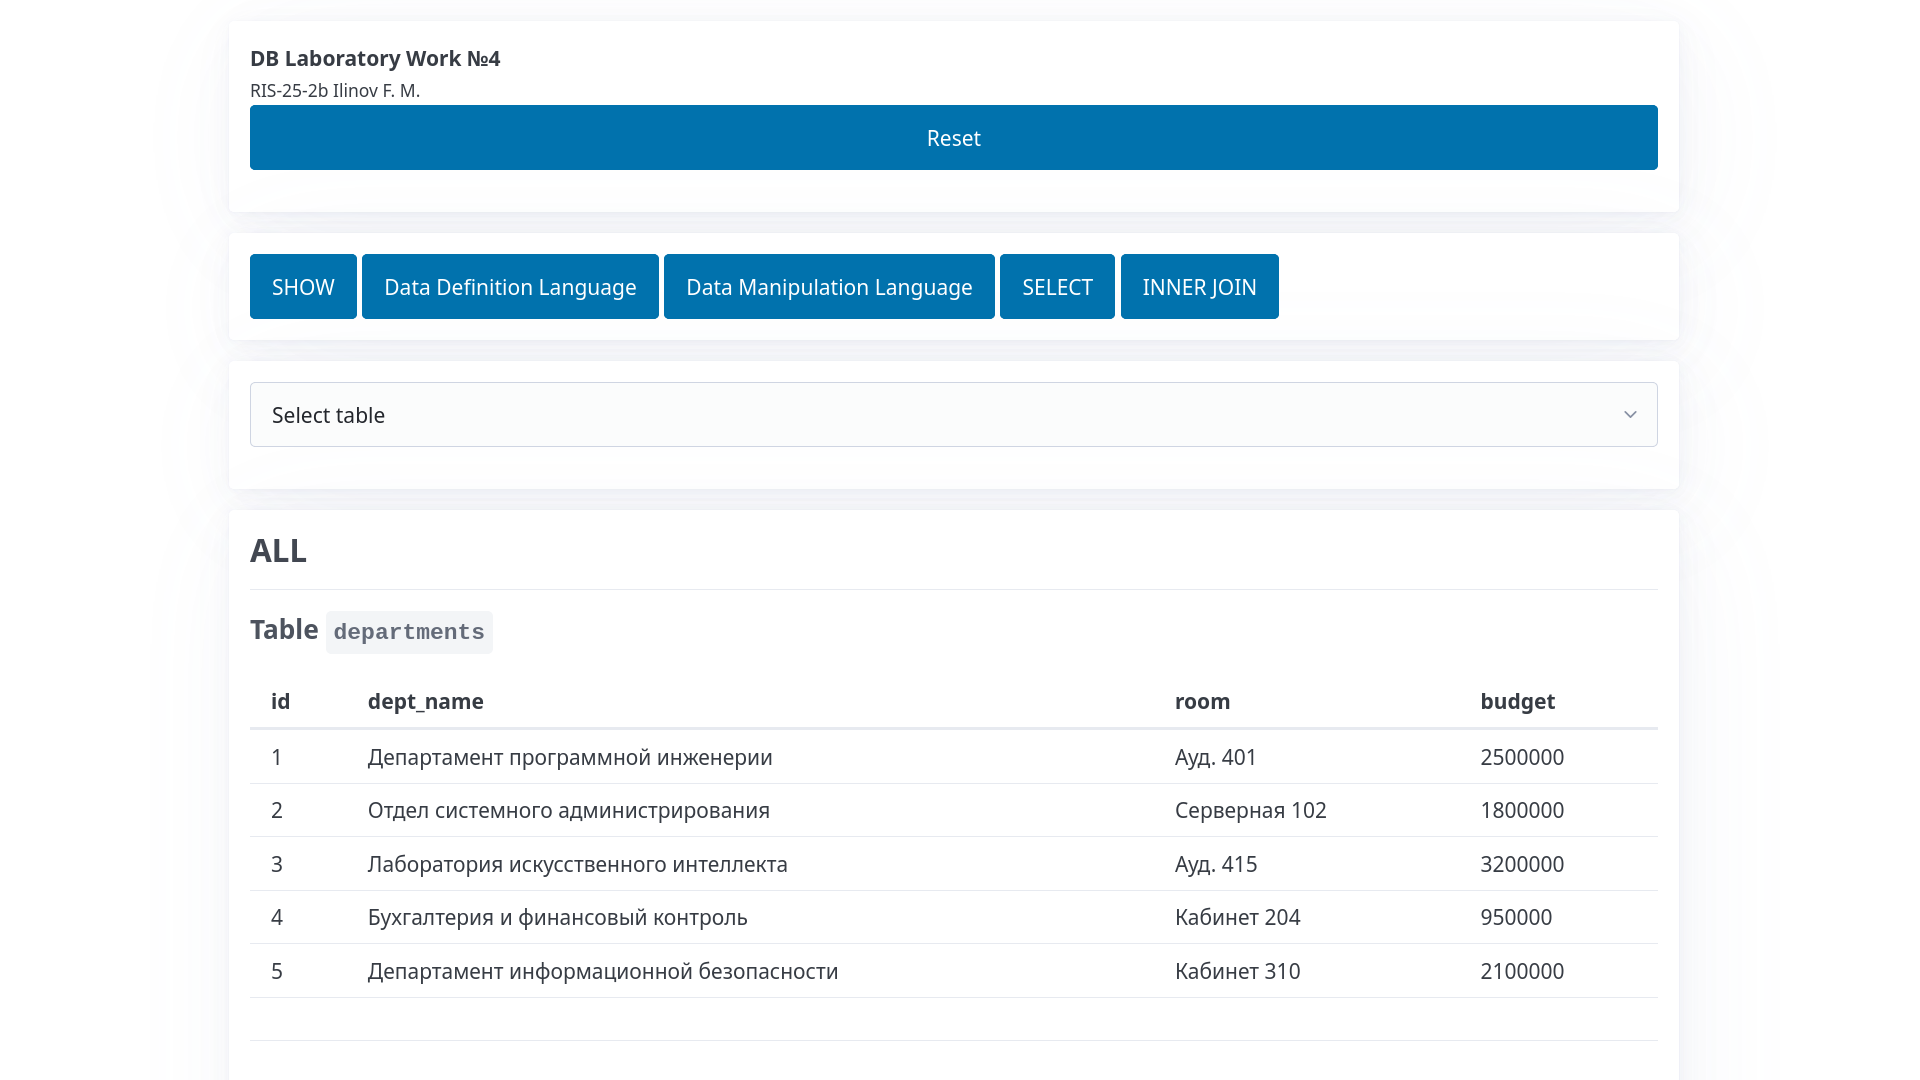
\includegraphics[width=\textwidth]{img_tables}
    \caption{Отображение списка таблиц и их кортежей в браузере}
    \label{fig:fig-tables}
\end{figure}

Снимок экрана создания новой таблицы с первичным и внешним ключами приведен на рисунке~\ref{fig:fig-ddl-create}.

\begin{figure}[H]
    \centering
    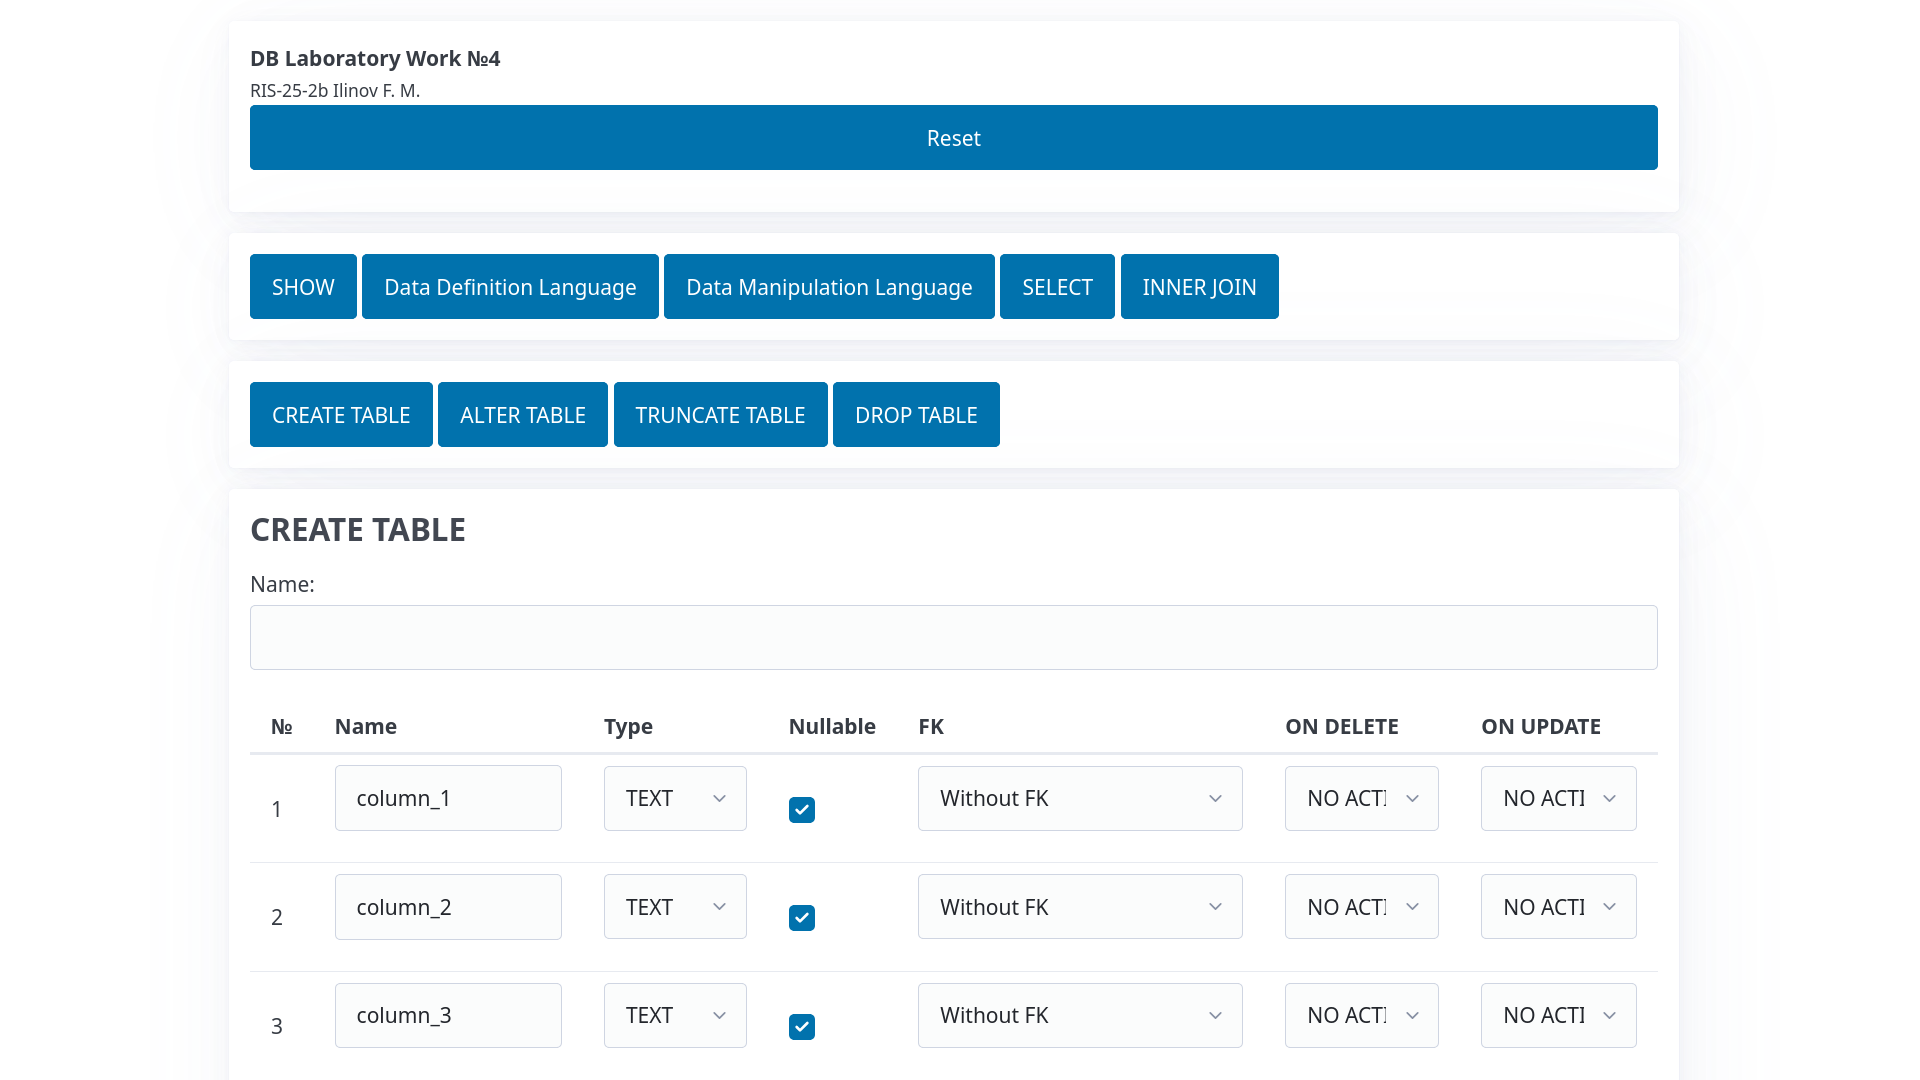
\includegraphics[width=\textwidth]{img_ddl_create}
    \caption{Создание таблицы через двухэтапную форму DDL}
    \label{fig:fig-ddl-create}
\end{figure}

Снимок экрана модификации колонок таблицы с помощью команды ALTER TABLE приведен на рисунке~\ref{fig:fig-ddl-alter}.

\begin{figure}[H]
    \centering
    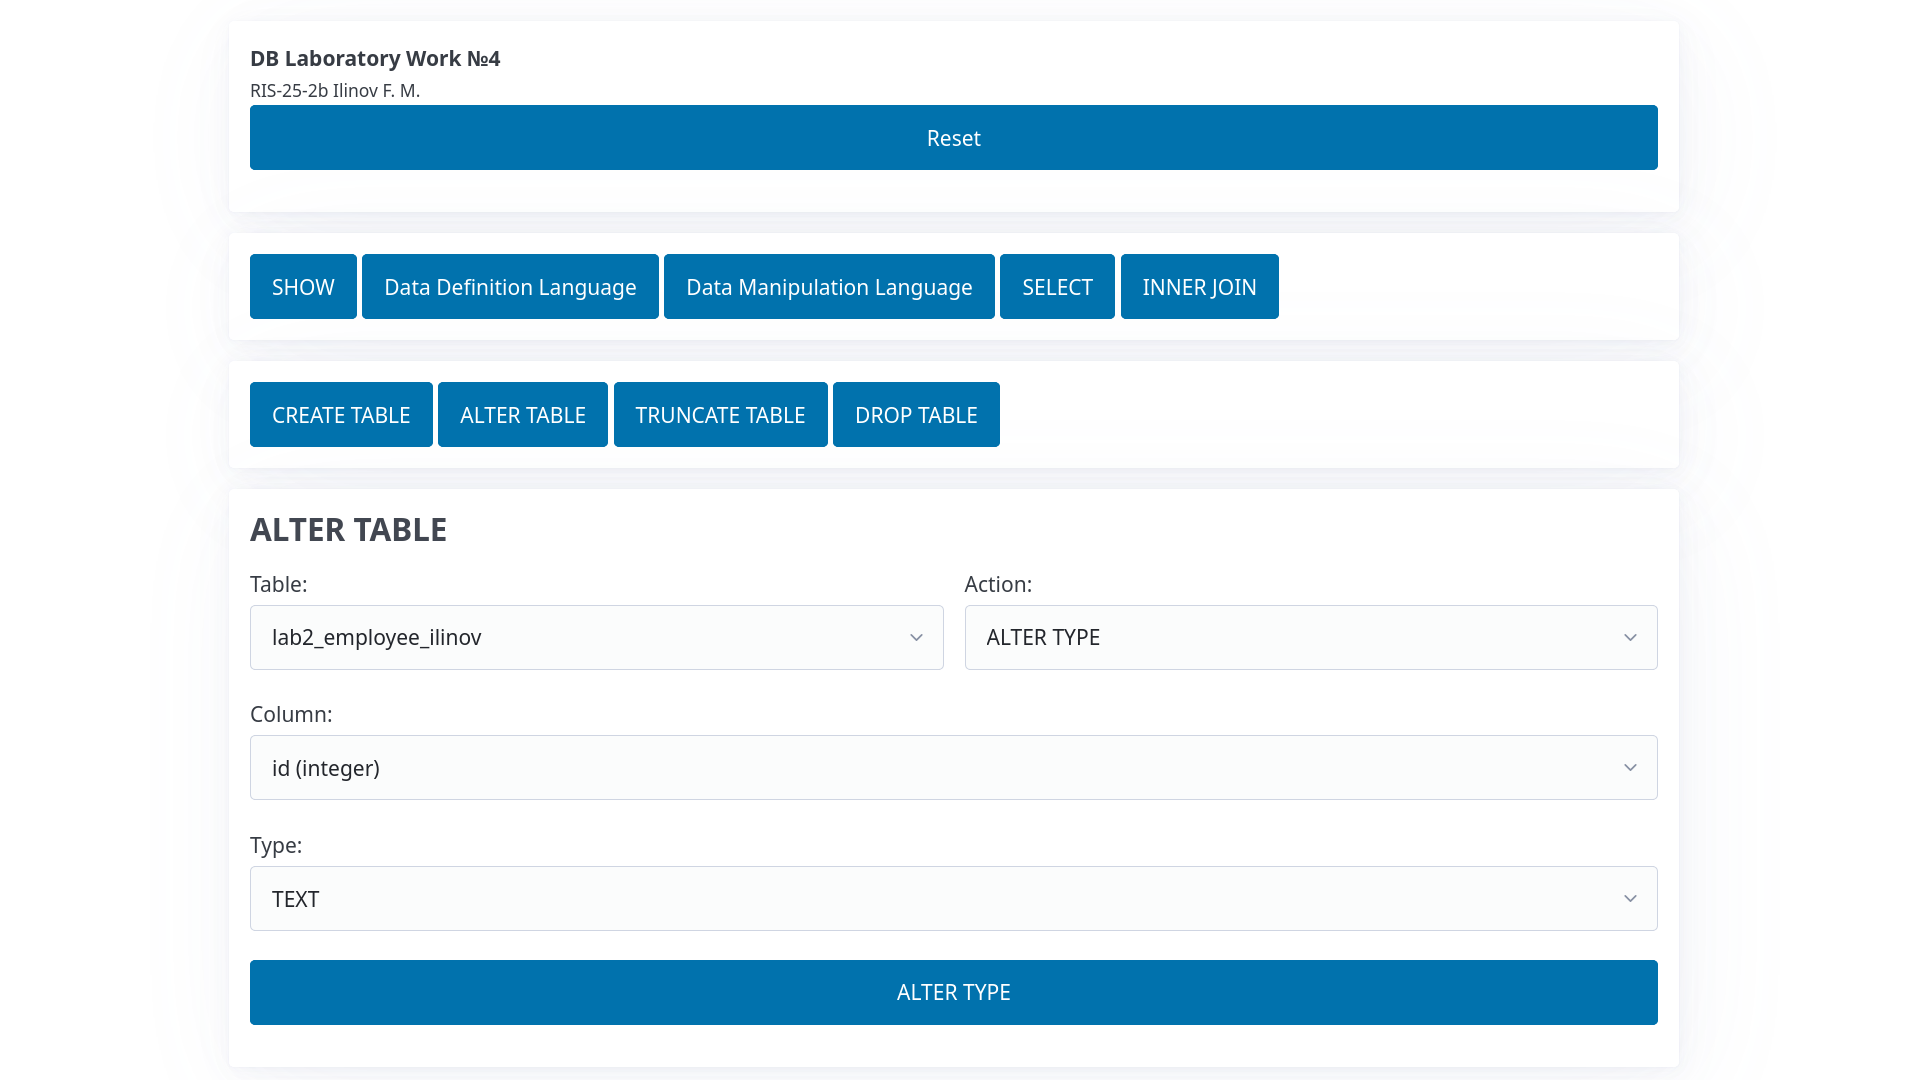
\includegraphics[width=\textwidth]{img_ddl_alter}
    \caption{Модификация структуры таблицы с помощью команды ALTER TABLE}
    \label{fig:fig-ddl-alter}
\end{figure}

Снимок экрана очистки данных таблицы оператором TRUNCATE представлен на рисунке~\ref{fig:fig-ddl-truncate}.

\begin{figure}[H]
    \centering
    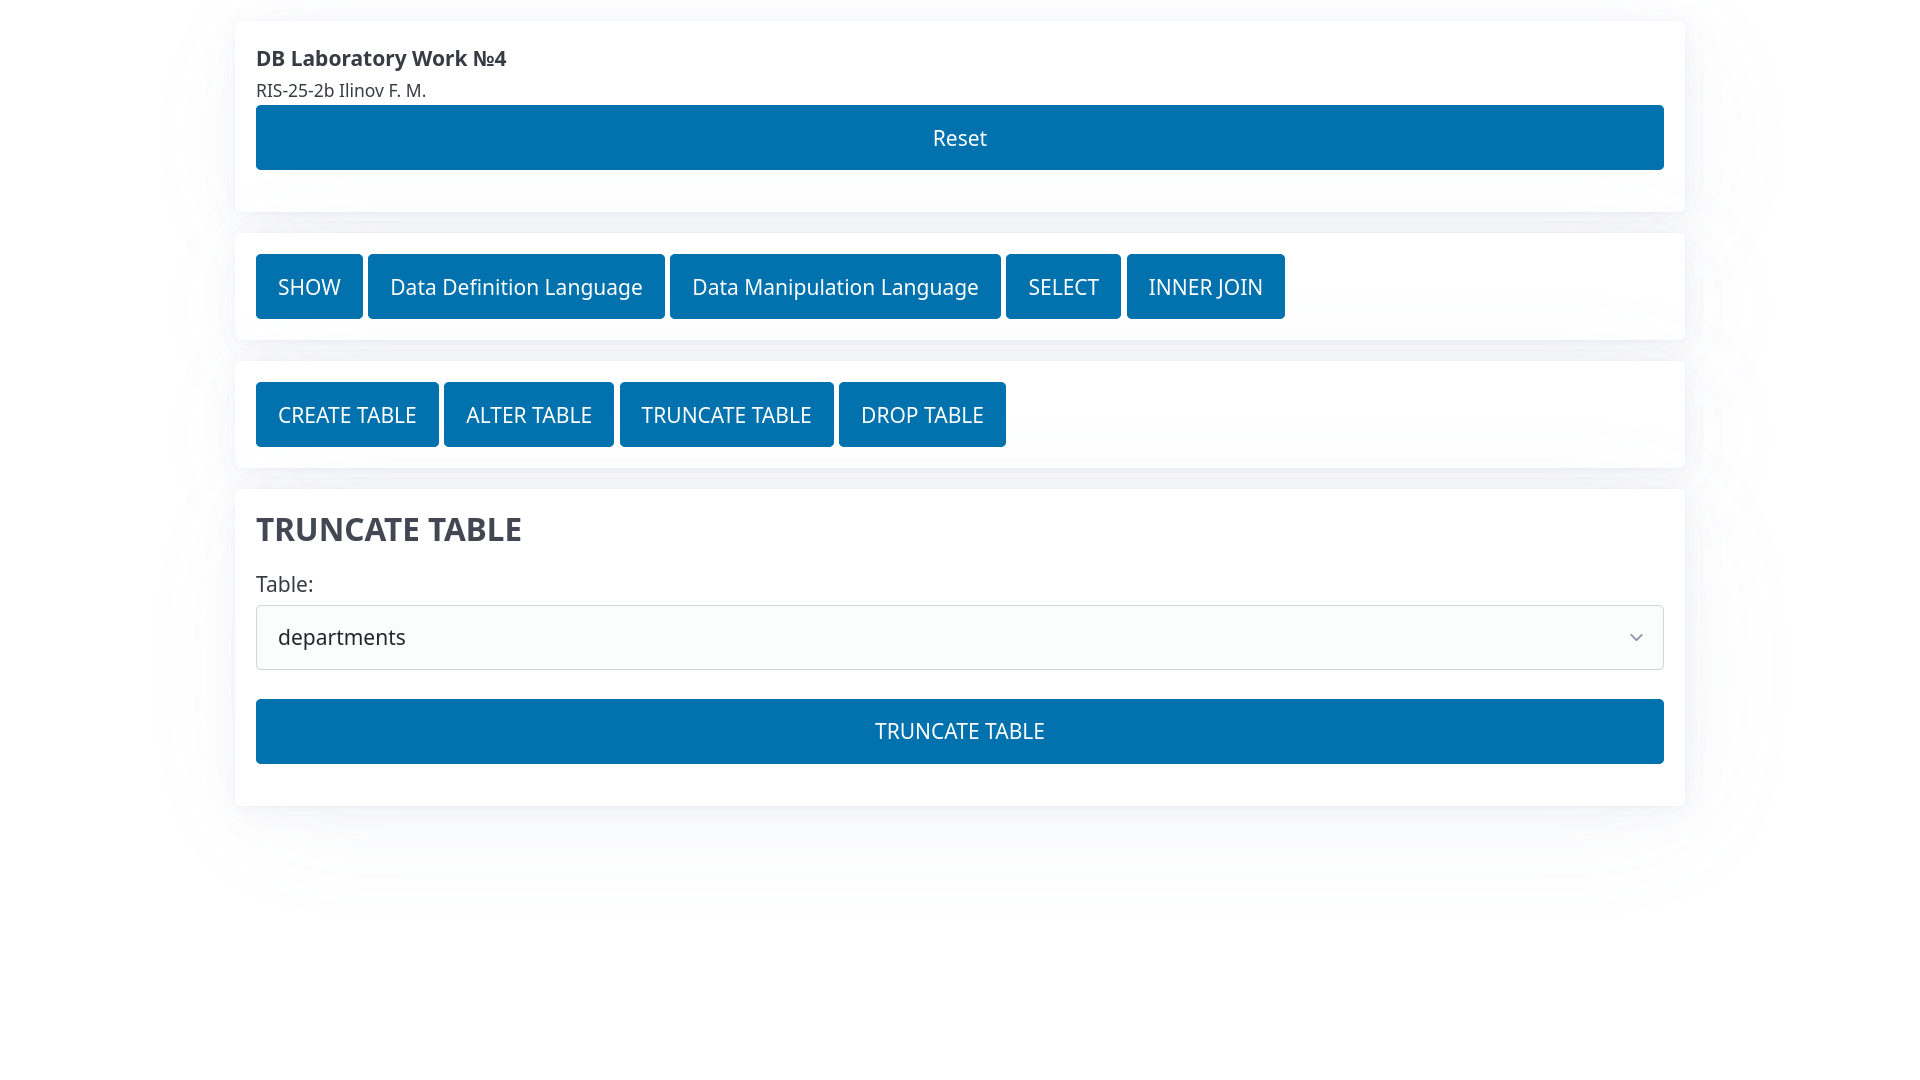
\includegraphics[width=\textwidth]{img_ddl_truncate}
    \caption{Очистка таблицы оператором TRUNCATE TABLE CASCADE}
    \label{fig:fig-ddl-truncate}
\end{figure}

Снимок экрана удаления таблицы с каскадной очисткой связей приведен на рисунке~\ref{fig:fig-ddl-drop}.

\begin{figure}[H]
    \centering
    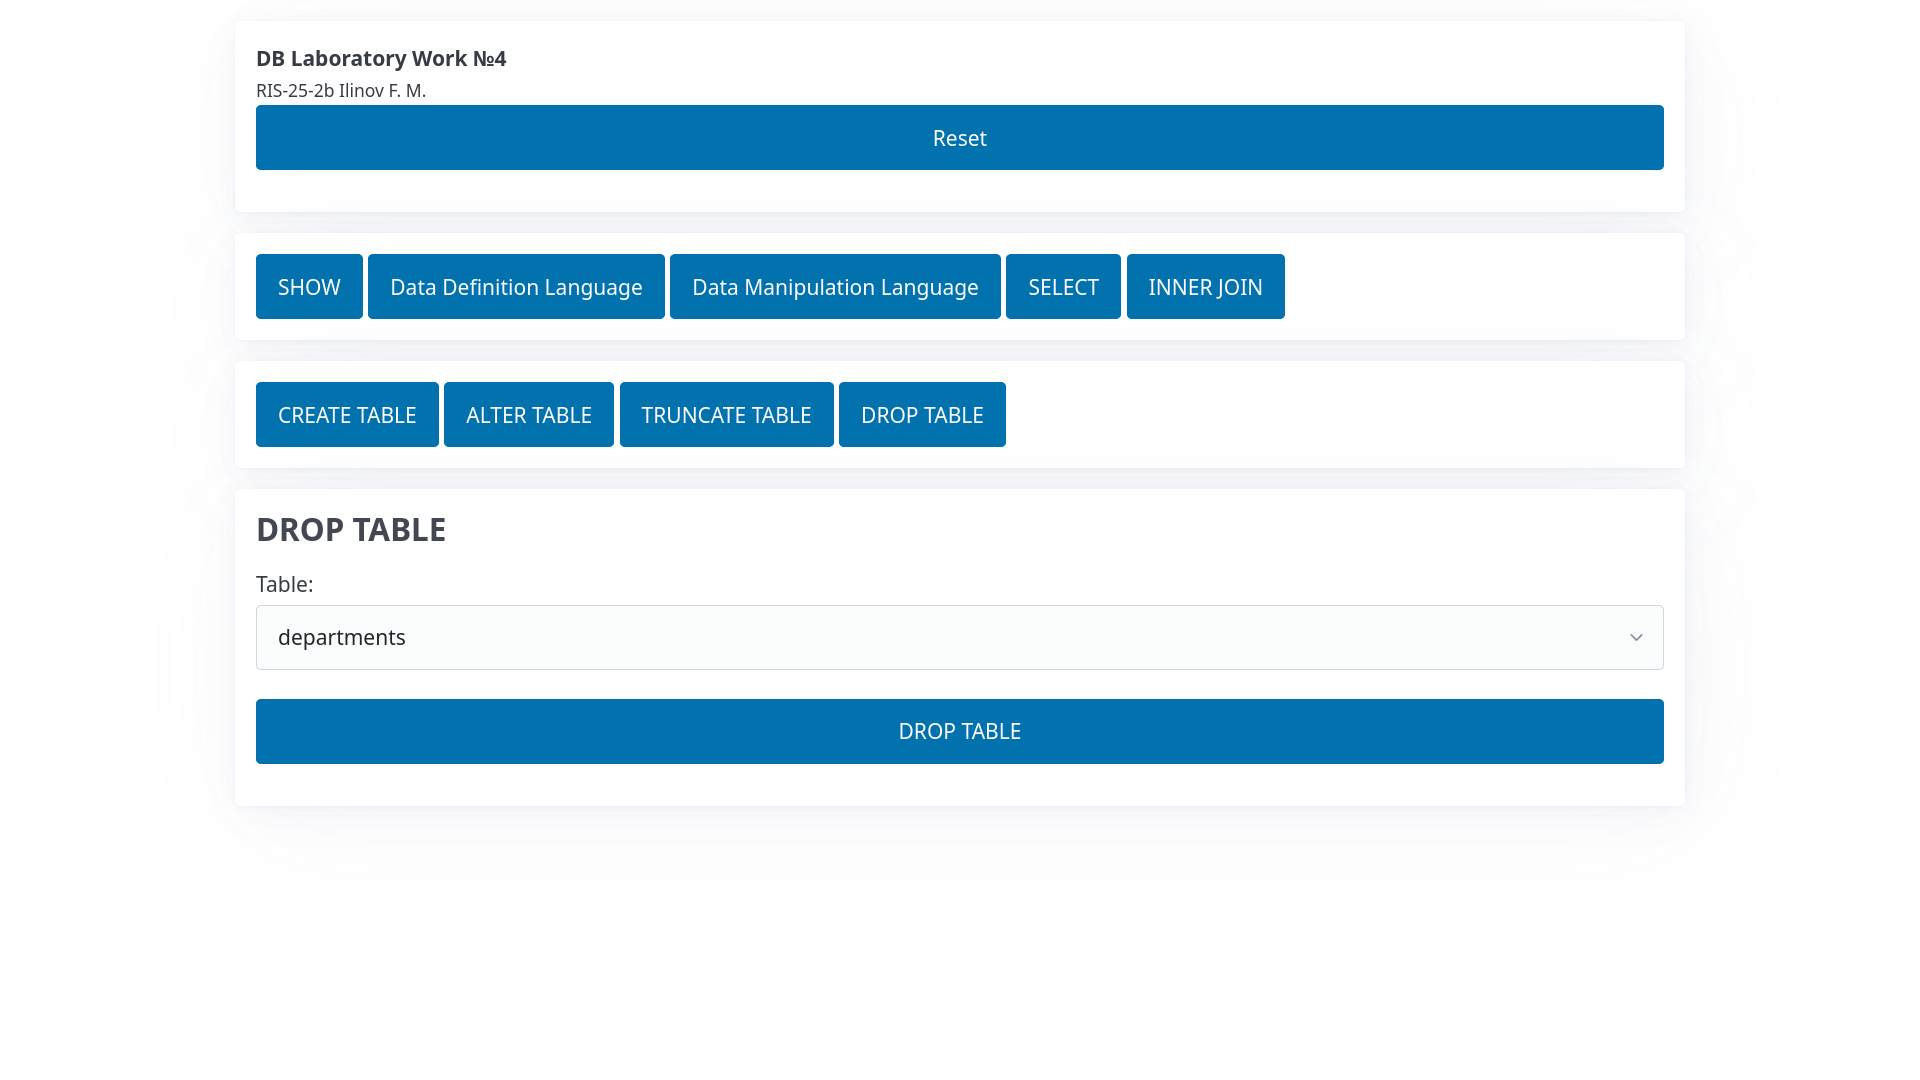
\includegraphics[width=\textwidth]{img_ddl_drop}
    \caption{Удаление сущности оператором DROP TABLE CASCADE}
    \label{fig:fig-ddl-drop}
\end{figure}

Снимок экрана пакетного добавления нескольких кортежей оператором INSERT INTO представлен на рисунке~\ref{fig:fig-dml-insert}.

\begin{figure}[H]
    \centering
    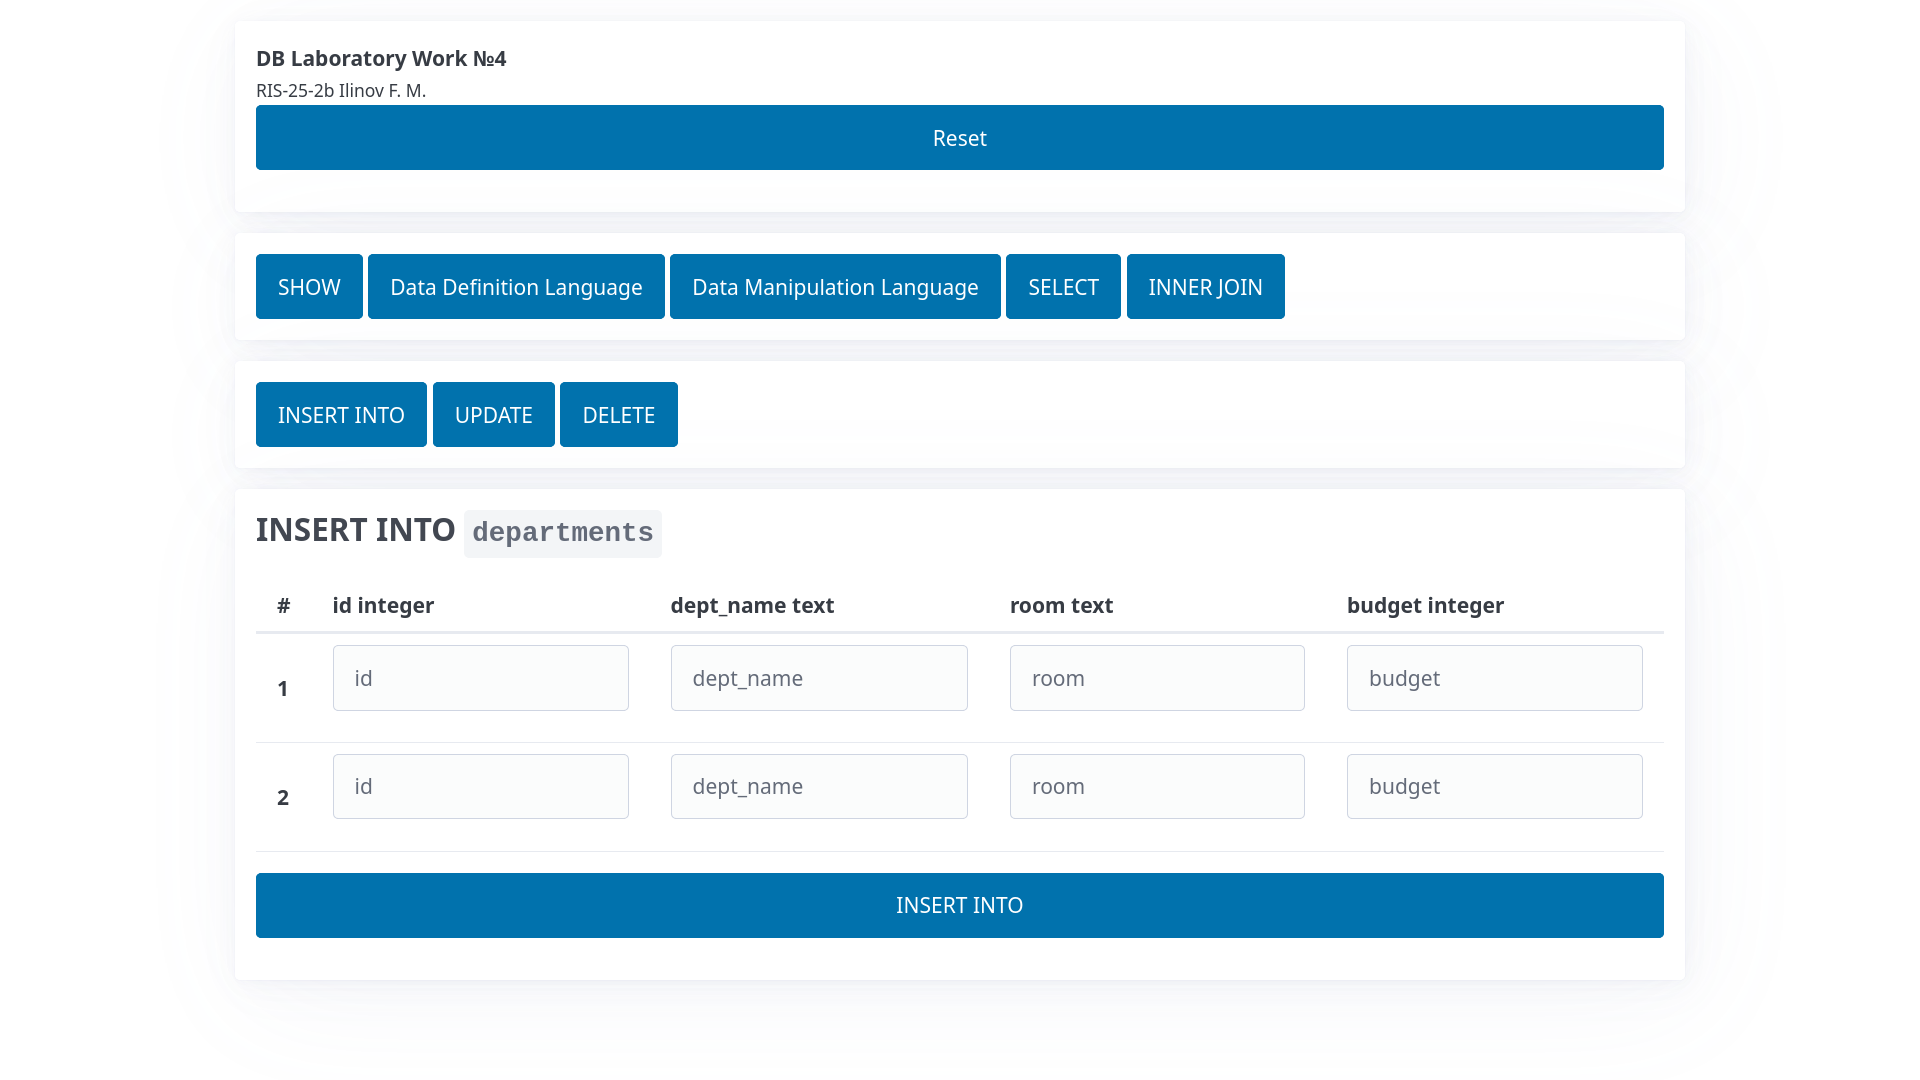
\includegraphics[width=\textwidth]{img_dml_insert}
    \caption{Пакетная вставка записей с помощью команды INSERT INTO}
    \label{fig:fig-dml-insert}
\end{figure}

Снимок экрана изменения данных оператором UPDATE с предикатом WHERE приведен на рисунке~\ref{fig:fig-dml-update}.

\begin{figure}[H]
    \centering
    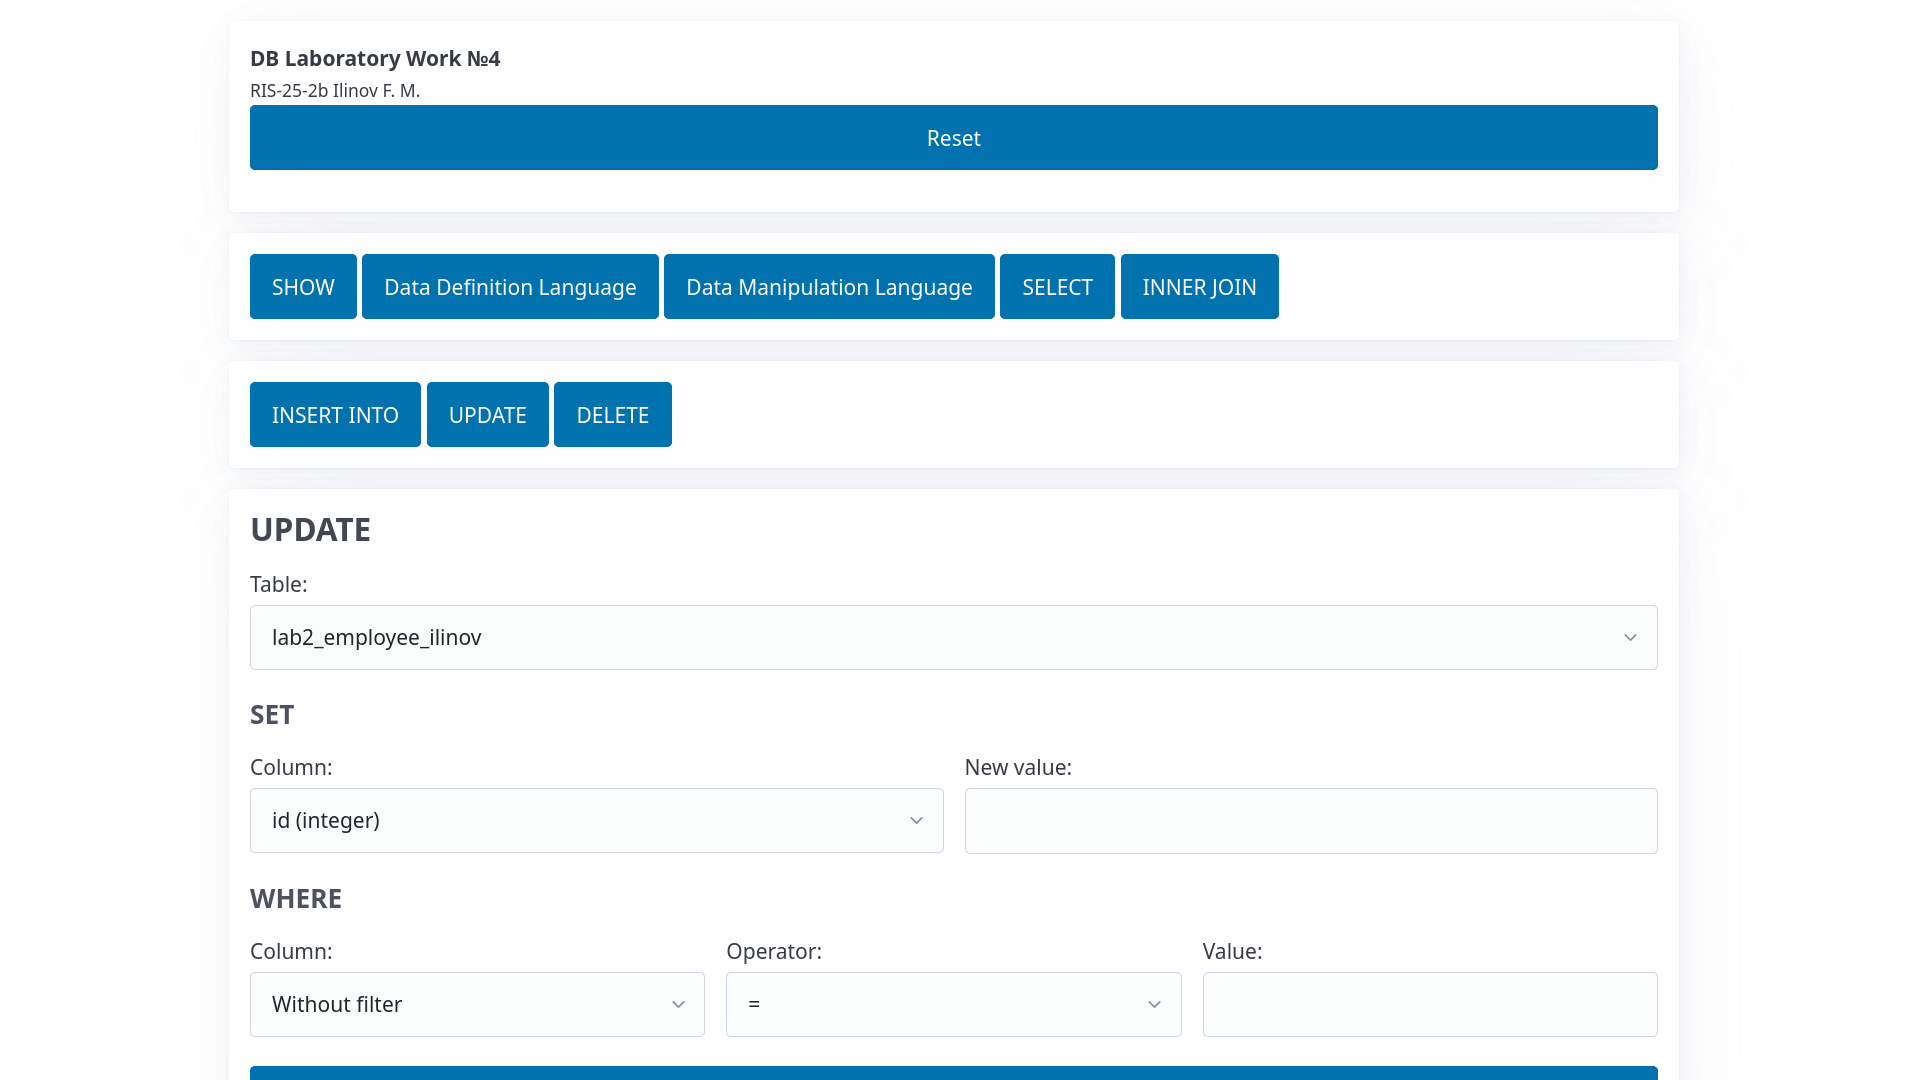
\includegraphics[width=\textwidth]{img_dml_update}
    \caption{Обновление данных с условием фильтрации}
    \label{fig:fig-dml-update}
\end{figure}

Снимок экрана удаления записей оператором DELETE приведен на рисунке~\ref{fig:fig-dml-delete}.

\begin{figure}[H]
    \centering
    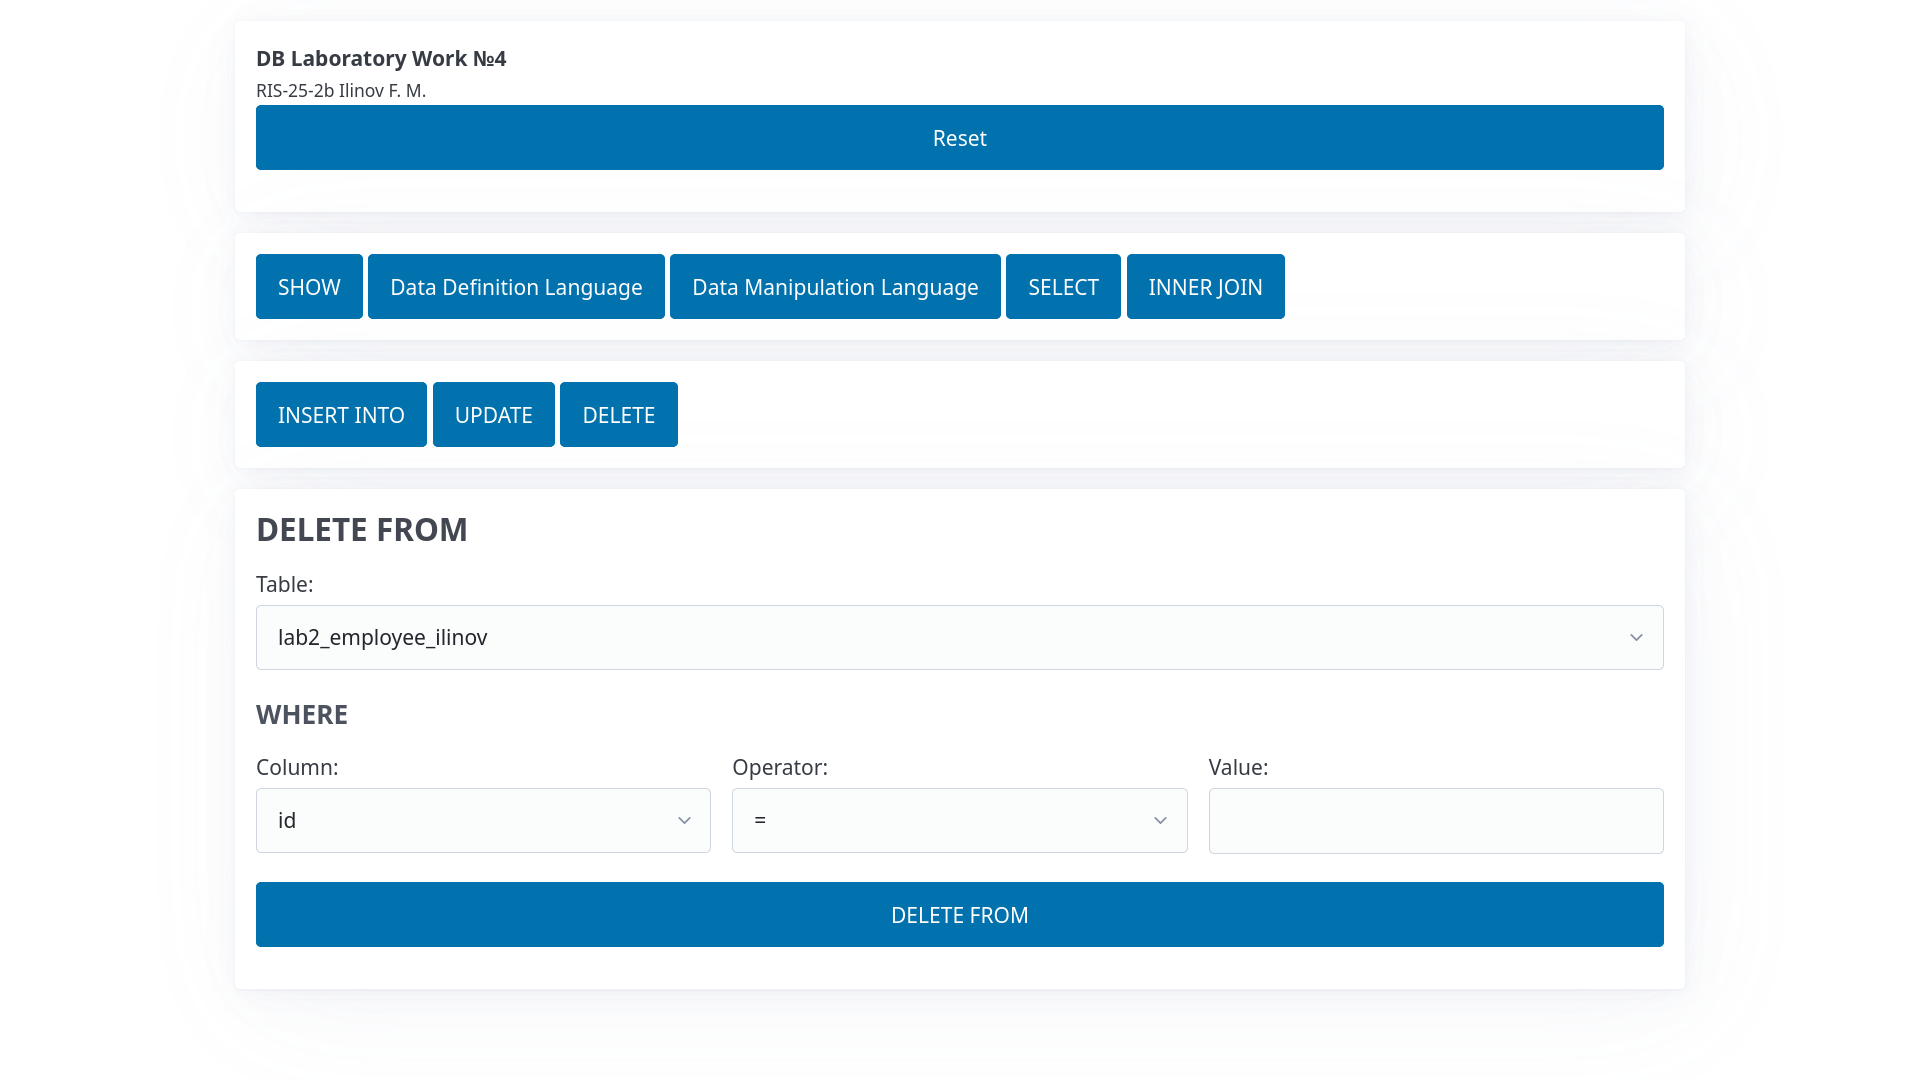
\includegraphics[width=\textwidth]{img_dml_delete}
    \caption{Удаление записей оператором DELETE FROM по условию}
    \label{fig:fig-dml-delete}
\end{figure}

Снимок экрана параметризованной выборки SELECT с фильтрацией и сортировкой приведен на рисунке~\ref{fig:fig-select}.

\begin{figure}[H]
    \centering
    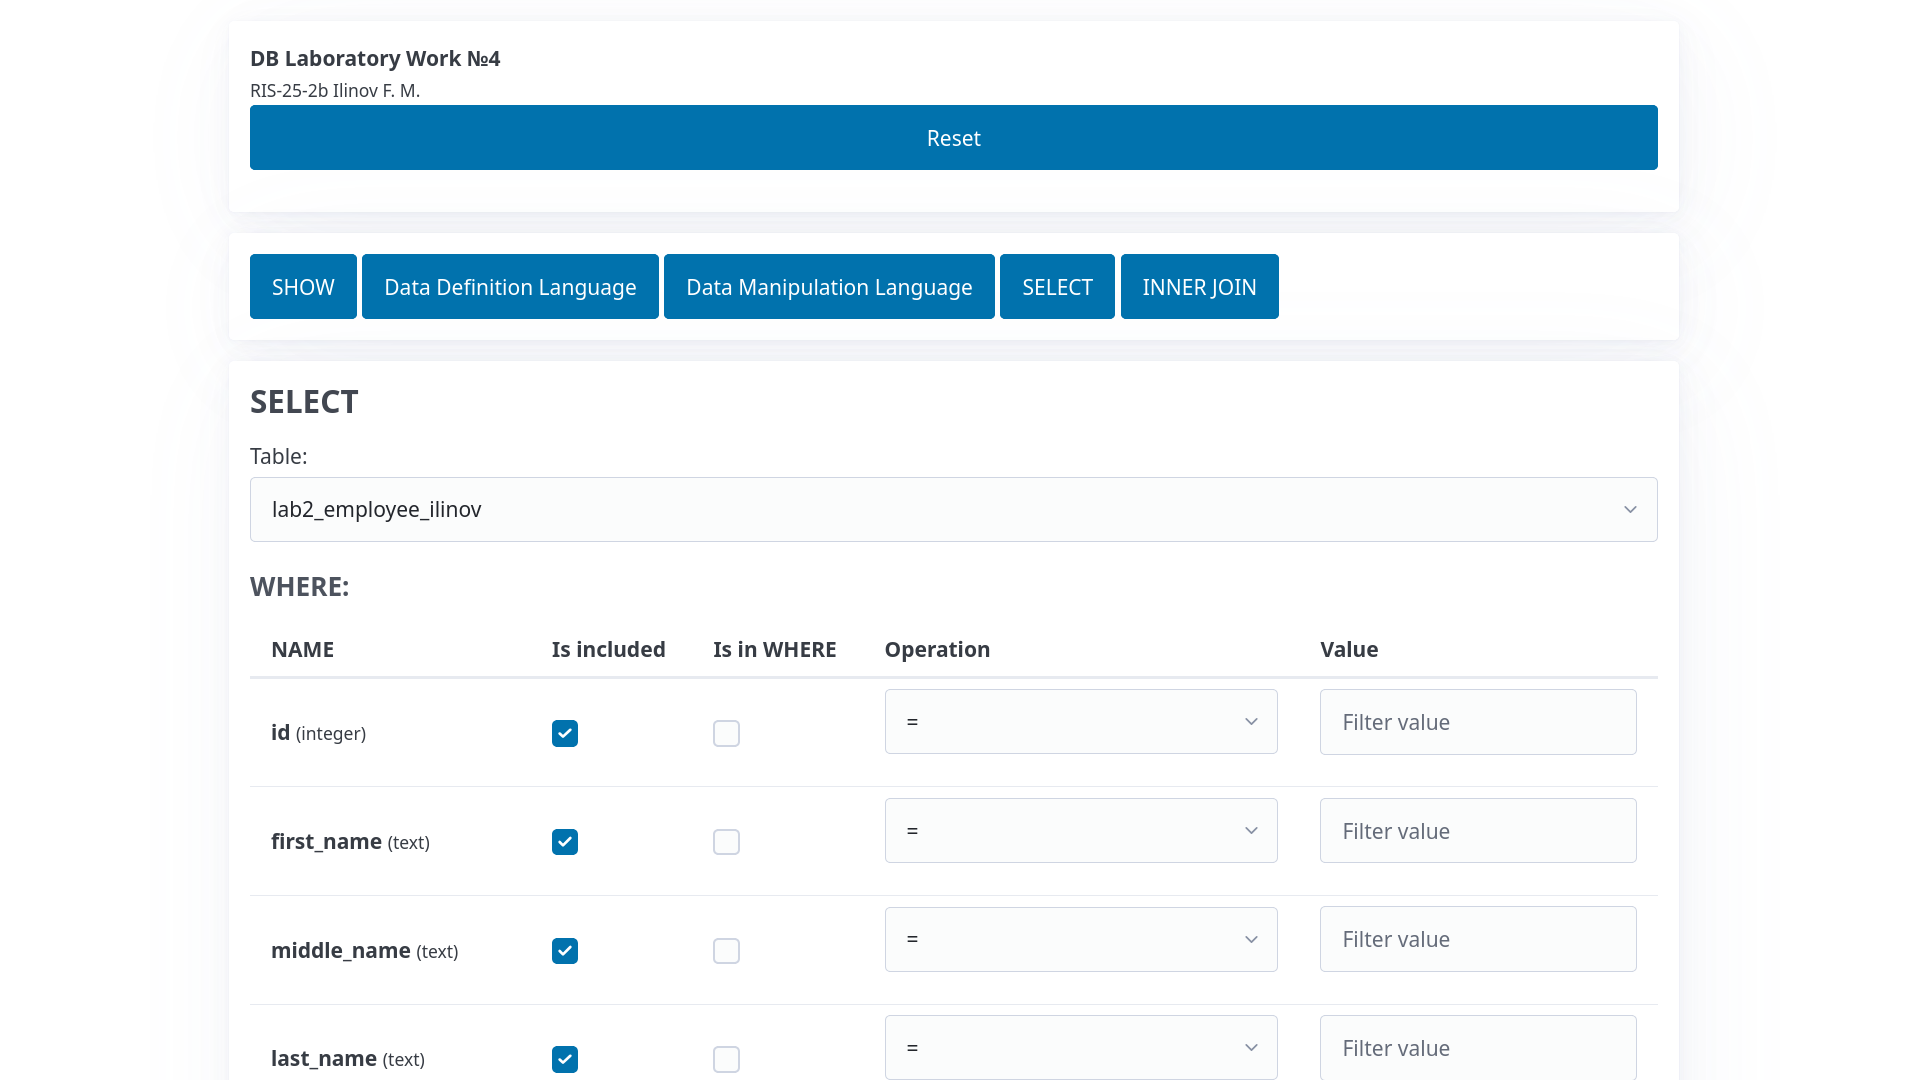
\includegraphics[width=\textwidth]{img_select}
    \caption{Результаты параметризованной выборки SELECT ... WHERE}
    \label{fig:fig-select}
\end{figure}

Снимок экрана внутреннего соединения двух таблиц оператором INNER JOIN представлен на рисунке~\ref{fig:fig-join}.

\begin{figure}[H]
    \centering
    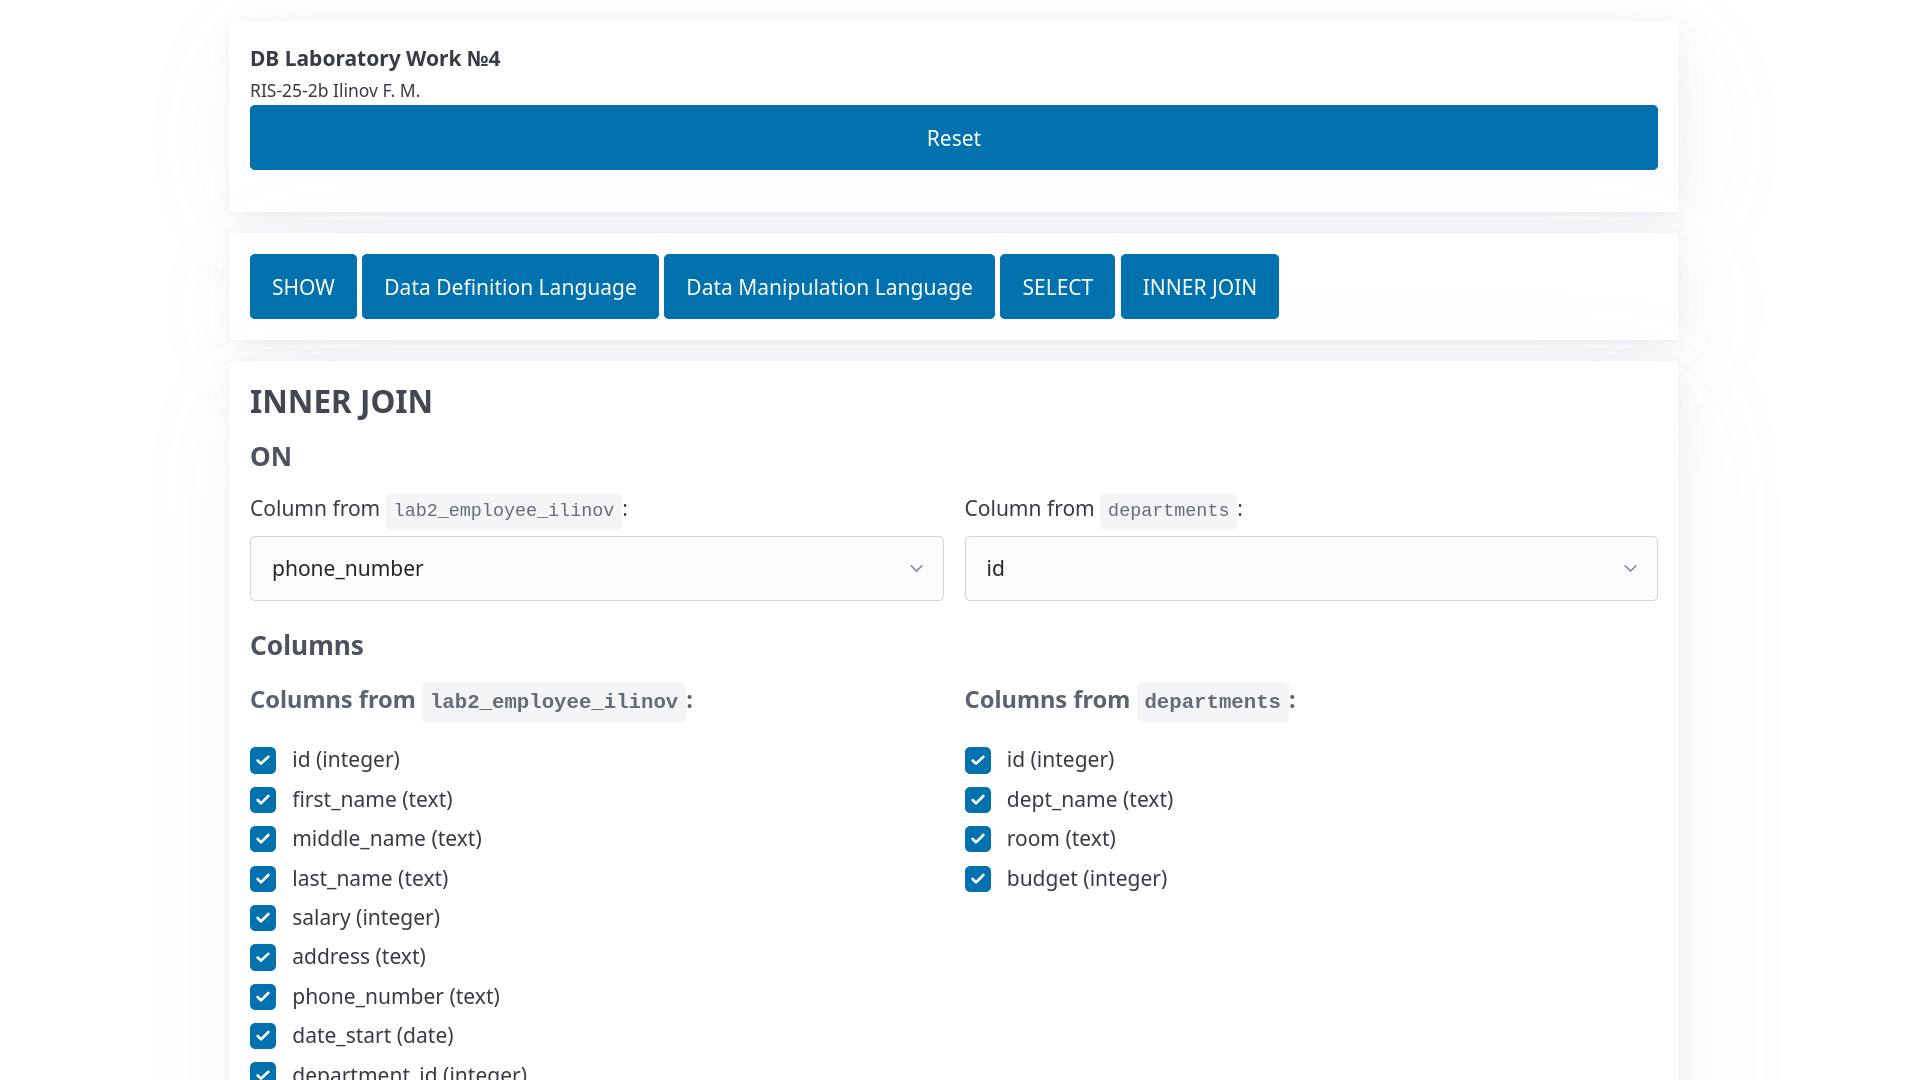
\includegraphics[width=\textwidth]{img_join}
    \caption{Результаты реляционного соединения INNER JOIN ... ON}
    \label{fig:fig-join}
\end{figure}

На всех этапах тестирования сформированные SQL-запросы корректно валидировались и исполнялись СУБД PostgreSQL, а результирующие наборы данных и системные уведомления в полном объеме выводились в веб-интерфейсе.


\backmatter % библиография и заключение

\Conclusion % заключение к отчёту
\label{cha:conclusion}

В ходе работы были решены следующие задачи:
\begin{enumerate}
    \item Разработан веб-сервер с модульной архитектурой и сквозным стеком вызовов от пользовательских HTML-форм до ядра СУБД PostgreSQL;
    \item Реализовано безопасное конструирование SQL-запросов с экранированием идентификаторов (\texttt{quoteIdent}) и литералов (\texttt{quoteLiteral});
    \item Реализована поддержка операций языка определения данных DDL: двухэтапное создание таблиц с поддержкой первичных и внешних ключей (включая самоссылающиеся ограничения), изменение структуры через ALTER TABLE, очистка через TRUNCATE и каскадное удаление через DROP TABLE CASCADE;
    \item Реализована поддержка операций языка манипулирования данными DML: пакетная вставка записей с автоматической обработкой NULL-значений, изменение данных по условию UPDATE и удаление данных DELETE;
    \item Реализован интерактивный конструктор запросов выборки SELECT с динамической проекцией, фильтрацией и сортировкой, а также оператор реляционного соединения INNER JOIN двух таблиц по общему ключу;
    \item Реализован механизм изоляции и быстрого восстановления исходного состояния базы данных через эндпоинт \texttt{POST /reset}.
\end{enumerate}

Корректность функционирования подтверждена серией тестов в браузере с прозрачным аудитом текста сформированных SQL-команд.


\bibliographystyle{ugost2008}
\bibliography{report-lab-04}


\end{document}
